\chapter{Implementación y Pruebas}\label{chapter:implementation}
La etapa de implementación del \textit{software} es el proceso de convertir una especificación del sistema en un sistema ejecutable. Esta fase comprende la materialización, en forma de código, de todos los artefactos, descripciones y arquitectura propuestos en la etapa de análisis y diseño; con el objetivo de conformar el producto final requerido por el cliente [\cite{91}].

Una vez desarrollado el \textit{software}, el mismo debe ser sometido a una serie de pruebas que muestren que el sistema se ajusta a su especificación y que cumple con las expectativas del usuario. Según [\cite{91}], esta etapa es conocida como la validación e implica una serie de procesos de comprobación, como las inspecciones y revisiones. Por lo que el presente capítulo tiene como objetivo documentar los resultados de las fases de implementación del sistema y de la estrategia de pruebas desarrollada, y validar la solución propuesta.

%El desarrollo de las vistas del nivel de presentación está compuesto por 
%componentes, piezas de código con un comportamiento específico que unidos crean 
%aplicaciones web [46], si estos se abstraen correctamente pueden ser reutilizables, 
%reduciendo el desarrollo repetitivo [47]

\section{Implementación}
Para el desarrollo de la aplicación web se ha utilizado un gran número de librerías y recursos externos para facilitar el desarrollo [\cite{47}]. Por ello no se van a explicar todos, sino los de más relevancia acorde a las secciones en las que se ha estructurado el proyecto, que son las que tienen que ver con el \textit{framework} Vue.
%En este apartado se comentan algunas de las partes de la implementación realizada para el desarrollo del prototipo con Vue 3.

%\section{Estructura del código}
%El código de nuestra aplicación sigue la estructura de proyecto predeterminada de Vue y la guía de estilo oficial [\cite{47}] (Figura 4.2).

%Como estamos construyendo un SPA, \textit{index.html} es el sitio de inicio y también el único archivo \textit{.html} en el directorio. Su cuerpo contiene un solo elemento <div id=``app'' </div>, donde se montará el componente raíz \textit{App.vue}. La Figura 4.3 muestra el árbol de componentes Vue de \textit{App.vue}.

%La Figura 3 muestra la estructura del proyecto y todas las carpetas y archivos se describen a continuación:
\begin{figure}[htbp]
\centering
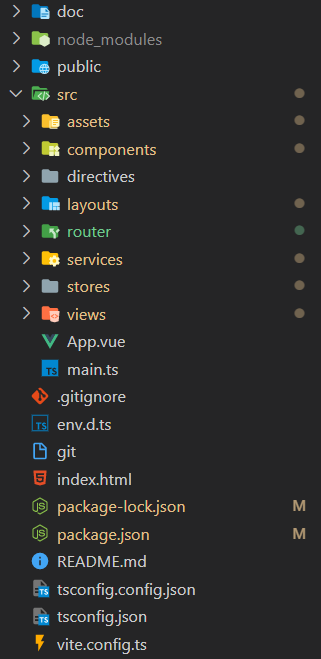
\includegraphics[scale=0.65]{Graphics/code}
\caption{Estructura del código.}
\label{fig:code}
\end{figure}

En la Figura \ref{fig:code} se muestra la estructura por carpetas y archivos usados para el desarrollo del nivel de presentación. La carpeta ``src'' almacena todos los archivos con el código para la creación de la aplicación; el resto de las carpetas y ficheros son configuraciones del proyecto, muy importantes para el desarrollo de este, pero no se van a explicar. Dentro de esta encontramos las distintas carpetas y archivos:

\begin{itemize}
\item \textbf{assets}: esta carpeta incluye los activos estáticos de la aplicación que pueden ser el logotipo de una empresa, imágenes, fuentes, entre otros.
\item \textbf{components}: esta carpeta contiene todos los componentes de la aplicación.
\item \textbf{directives}: esta carpeta contiene todas las directivas de la aplicación.
\item \textbf{layouts}: contiene los componentes que se encargan del diseño visual de la interfaz.
\item \textbf{router}: contiene todas las rutas que muestran las vistas.
\item \textbf{services}: contiene todos los servicios y definiciones de la aplicación.
\item \textbf{stores}: contiene todos los \textit{stores} creados mediante la biblioteca Pinia.
\item \textbf{views}: contiene todas las vistas de la aplicación.
\item \textbf{App.vue}: este archivo es el componente raíz donde se anidan todos los demás componentes. Este archivo es responsable de manejar todos los componentes.
\item \textbf{main.ts}: archivo encargado de cargar la aplicación. En él se adjuntan las librerías principales, como Pinia y el archivo principal (App.vue).
\end{itemize}

\subsection{Componentes}
Cada \textit{framework} tiene su propia manera de definir los componentes y realizar su propia interpretación de estos. En Vue se pueden definir de varias formas, una de ellas  es la llamada componentes de un solo archivo o en inglés \textit{Single File Components}. Estos componentes nos permiten, como su nombre indica, encapsular el código CSS, HTML y TypeScript en un único archivo.

Esto es un modo muy útil de definir los componentes puesto que cuando la aplicación escale en tamaño nos será más fácil encontrar el código deseado y reduciremos en gran medida el tamaño en archivos del proyecto.

\begin{lstlisting}[language=C,caption={Código del archivo App.vue}, label={lst:app}]
<template>
    <component :is="$route.meta.layout || 'div'">
        <router-view></router-view>
    </component>
</template>

<script lang="ts">
import { defineComponent } from 'vue'
import { CmpSideBarMenu } from '@/components'

export default defineComponent({
    name:       'Application',
    components: {
        CmpSideBarMenu
    }
})
</script>

<style lang="scss">
@import "assets/sass/black-dashboard";
@import "assets/css/fontawesome5.css";
@import "assets/css/nucleo-icons.css";

// from node_modules libs
@import "vue-toastification/dist/index.css";
@import "nprogress/nprogress.css";
</style>
\end{lstlisting}

En \ref{lst:app} se puede observar el código del archivo principal de la aplicación desarrollada denominado ``App.vue''. El archivo, al igual que los archivos ``.vue'' de este proyecto, est'a dividido en tres secciones:
\begin{itemize}
\item <template>, dónde incorporamos el código HTML
\begin{itemize}
\item En esta sección hacemos uso de los componentes reutilizables, alguno de ellos con renderización condicional usando ``v-if''.
\end{itemize}
\item <script>, dónde encontramos el código TypeScript. En este apartado nos encontramos con lo siguiente:
\begin{itemize}
\item Importación de bibliotecas y componentes a utilizar.
\item components, sección dónde se realiza el registro de los componentes que se van a utilizar en el actual.
\item Composition API, el cambio más característico de la versión 3 de Vue, lo utilizamos con la función setup(), la cual se ejecuta al inicializar el componente. En el return de la función devolvemos todos aquellos objetos o funciones que queramos usar en el componente.
\item Ciclo de vida, usamos onMounted() para inicializar algunas propiedades que requieren tener valor nada más haya sido montado el componente.
\item Propiedades computadas, computed() cachea los datos hasta que los valores de las variables reactivas con las que se conforma no cambien. Esto nos evita realizar cálculos innecesarios.
\item Pinia, useStore se implementa para tener una gestión de estados centralizada.
\end{itemize}
\item <style>, dónde se implementa el CSS de la página.
\end{itemize}

Para la aplicación, usamos una plantilla personalizada por el cliente, en la cual existían componentes ya definidos para los principales elementos de una página Web como la barra de navegación, los botones, campos de entrada de datos, entre otros.

\subsection{Vistas}
Las vistas en Vue no son más que componentes que representan una página y por tanto se utilizarán de forma diferente. Estos componentes especiales llamados vistas, se encargan de montar una estructura de componentes reutilizables, y además de encargarse de gestionar los datos necesarios que puedan requerir para suministrárselos a unos componentes u a otros, definiendo de esta manera las relaciones entre los mismos.

%poner codigo de tablas de certificados

Tanto los componentes como las vistas se comunican con todas las demás entidades ubicadas en el lado del cliente. Esto se debe a que esos son los archivos que el usuario verá e interactuará. Siempre que un usuario quiera navegar de una vista a otra, debe hacer uso de las rutas que están definidas en la carpeta \textit{router} y las funciones proporcionadas por la biblioteca Vue-Router. Cuando un usuario quiera crear, leer, modificar o eliminar datos, debe hacerlo a través de las funciones proporcionadas por la biblioteca Axios que envían solicitudes al servidor. Luego, cuando el servidor envía una respuesta al \textit{frontend}, se almacena en la entidad de la \textit{store} de Pinia. Si un usuario desea obtener información, ejecuta métodos captadores ubicados en la entidad \textit{store} de Pinia que recuperan la información solicitada. Todas estas entidades se explicarán detalladamente en sus respectivas secciones.

En esta sección, daremos una breve descripción de la vista ViewListUsers.vue, la cual muestra la lista de usuarios del sistema. A continuación se muestra un fragmento de código de la sección <script> de esta vista:

\begin{lstlisting}[language=C,caption={Sección <script> de VueListUsers.vue}, label={lst:viewlist}]
<script lang="ts">
export default defineComponent({
    name: 'ViewListUsers',
    components: {
        CmpCard,
        CmpDataTable
    },
    setup() {
        //#region ======= DECLARATIONS & LOCAL STATE ==========================================
        const usersStore = useUsersStore()
        const eMode: EntityTypes = EntityTypes.Users
        const router = useRouter()
        const toast = useToast()
        const columns = HUsersTable
        const { tfyBasicSuccess, tfyBasicFail } = useToastify(toast)
        //#endregion ===========================================================

        //region ======== HOOKS ================================================
        onMounted(() => {
            // populate users datatable
            usersStore.reqUsersPages(queryBase).catch(err => tfyBasicFail(err, 'Users', 'request'))
        })

        //endregion ============================================================
        
        //#region ======= EVENTS HANDLERS ======================================
        function h_navCreateUsers() {
            router.push({
                name  : RoutePathNames.usersForm,
                params: {
                    fmode: 'create' as TFormMode,
                    id   : '',
                    cname: RoutePathNames.usersCreate 
                }
            })
        }
        //#endregion =========================================================

        return {
            eMode,
            columns,
            usersStore,
            h_navCreateUsers,
        }
    }
})
</script>
\end{lstlisting}

En este fragmento solo se muestran aquellas funciones y variables relacionadas a mostrar lista de usuarios y los eventos lanzados para navegar a la vista de crear usuario. Para obtener la lista de usuarios, al ser montado el componente, realizamos una petición al servidor a través de las funciones de Pinia, las cuales obtienen la lista y la guardan su estado. La función h\_navCreateUsers se encarga de manejar el evento lanzado cuando el usuario quiere navegar a la página de creación de usuarios mediante el uso del \textit{router}. Tanto la lista de usuarios guardada en Pinia, como las funciones que manejan los distintos eventos se las suministramos al componente CmpDataTable, el cual nos permite listar los usuarios en una tabla con funciones de paginado, y con distintos botones para las posibles acciones de gestión de usuarios.

\begin{lstlisting}[language=C,caption={Sección <template> de ViewListUsers.vue}, label={lst:viewlist1}]
<template>
    <transition appear name="page-fade">
        <div class="row">
            <div class="col-12">
                <CmpCard>
                    <CmpDataTable table-type="hover"
                                  :subject="$t('entities.users.name')"
                                  :entityMode="eMode"
                                  :columns="columns"
                                  :data="usersStore.getUsersList"
                                  :count="usersStore.getEntitiesCount"
                                  :has-actions="true"
                                  @navCreateIntent="h_navCreateUsers"
                                  @requestIntent="h_reqQuery"
                                  @editIntent="h_navEditUsers"
                                  @detailsIntent="h_navUserDetails"
                                  @deleteIntent="h_reqDeleteUser"
                    >
                    </CmpDataTable>
                </CmpCard>
            </div>
        </div>
    </transition>
</template>
\end{lstlisting}

El fragmento de código \ref{lst:viewlist1} muestra como fue implementado la sección <template> de ViewListUsers.vue, es en esta sección donde utilizamos el componente CmpDataTable. El resultado obtenido se puede observar en la Figura \ref{fig:usersList}.

\begin{figure}[htbp]
\centering
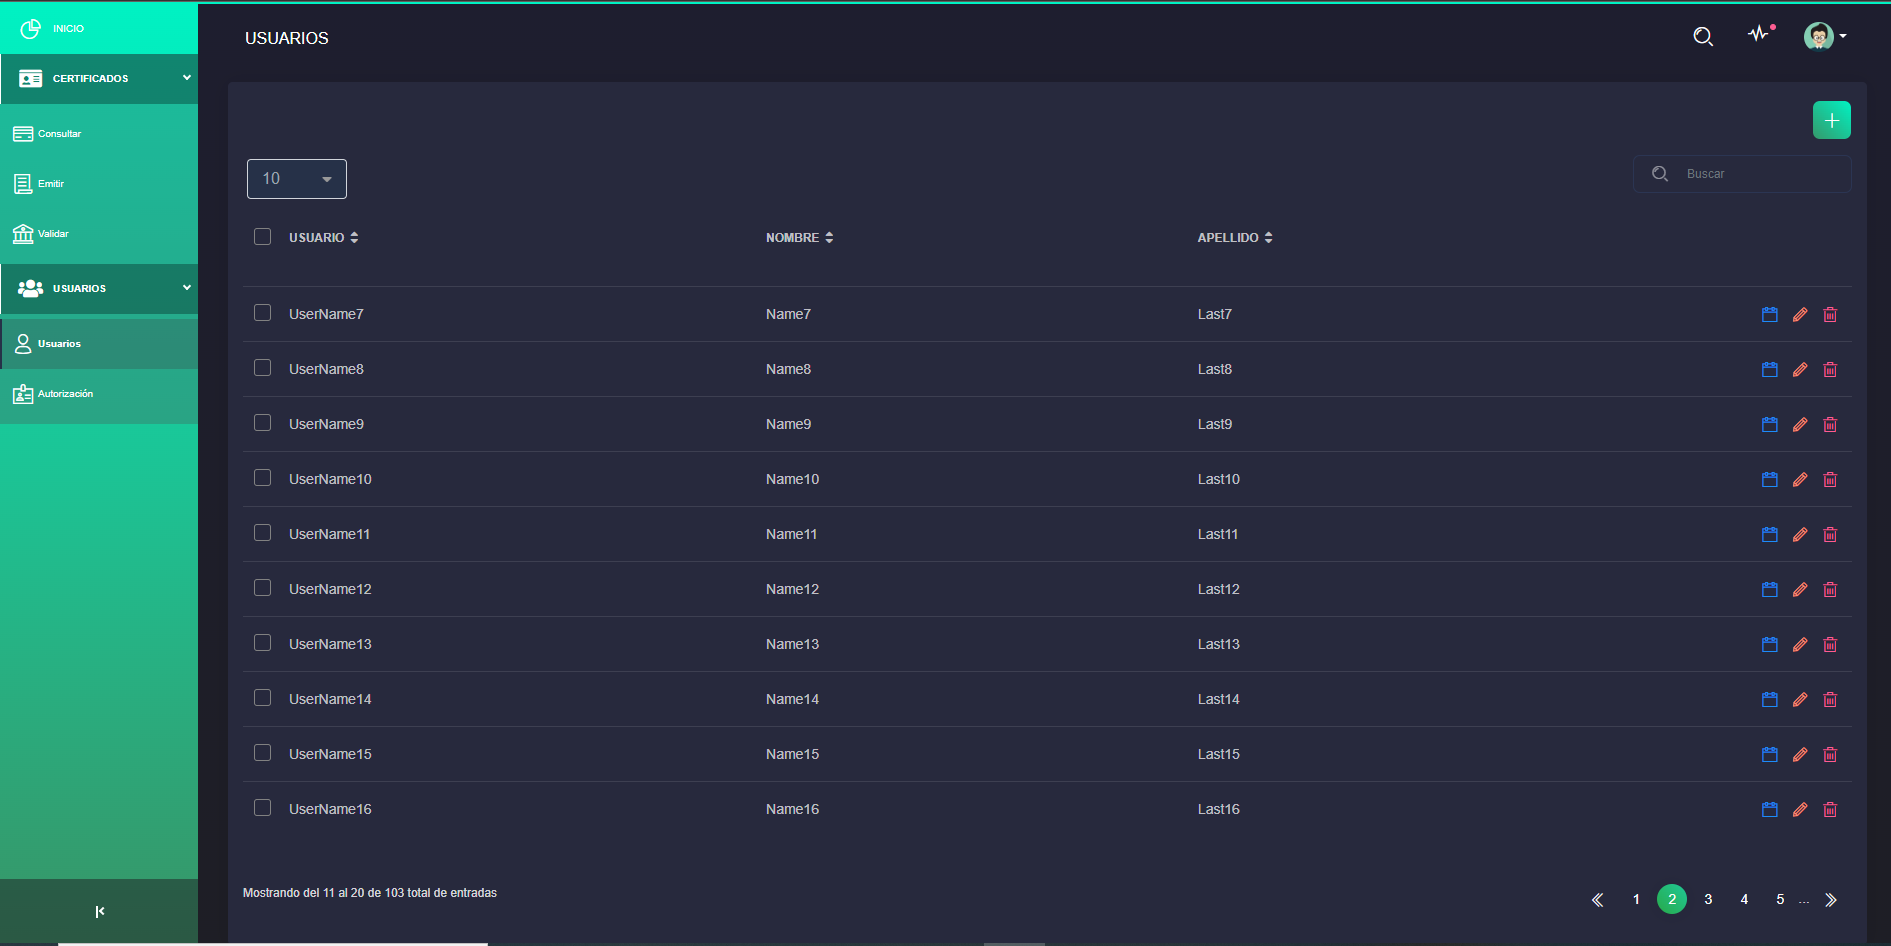
\includegraphics[width=\textwidth]{Graphics/usersList}
\caption{Vista de los usuarios.}
\label{fig:usersList}
\end{figure}

\subsection{Router}
El \textit{router} es una pieza fundamental de las SPA y por lo tanto es una pieza que no puede faltar en ningún \textit{framework} completo. Un \textit{router} es el elemento \textit{software} encargado de relacionar una URL a una vista, de manera que cuando se escriba una URL en el navegador, automáticamente se visualizara la vista relacionada. Además, un router debe proveer de diferentes herramientas para poder enviar datos dinámicos a las vistas y para establecer un sistema de permisos.

Vue viene con una biblioteca integrada que maneja el enrutamiento. Al crear un proyecto Vue, se genera automáticamente una carpeta de \textit{router} con un archivo index.ts con una configuración de ruta completa. Para definir nuevas rutas, simplemente podemos agregar un objeto al arreglo de rutas. El objeto consta de tres atributos:

\begin{itemize}
\item ruta: La URL para acceder a la ruta.
\item nombre: El nombre de la ruta. Utilizado como referencia a la ruta en ciertas funciones.
\item componente: El archivo que representa esta ruta.
\end{itemize}

En el campo del componente, podemos especificar el nombre del archivo directamente en el atributo del componente o pasarlo a una función que implemente \textit{lazy-loading}. La función extrae el código de la ruta del paquete ts y crea un fragmento separado para él. Este fragmento de código solo se carga cuando un usuario ingresa a la ruta. Es fácil de implementar y mejora significativamente el rendimiento de la aplicación.

El fragmento de código \ref{lst:router} muestra el \textit{router} de nuestra aplicación, donde además de las rutas básicas relacionadas con el inicio de sesión y la página inicial, añadimos las rutas relacionadas a los usuarios y los certificados. 

\begin{lstlisting}[language=C,caption={Configuración de las rutas}, label={lst:router}]
const router = createRouter({
    history: createWebHistory(import.meta.env.BASE_URL),
    routes:  [
        {
            path:      RoutePaths.login,
            name:      RoutePathNames.login,
            component: () => import('../views/auth/ViewLogin.vue'),
            meta:      { layout: LayBasePage }
        },
        {
            path:      RoutePaths.dashboard,
            name:      RoutePathNames.dashboard,
            component: () => import('../views/ViewDashboard.vue'),
            meta:      { layout: LayBaseDashboard }
        },
        {
            path:      RoutePaths.profile,
            name:      RoutePathNames.profile,
            component: () => import('../views/auth/ViewProfile.vue'),
            meta:      { layout: LayBaseDashboard , reqAuth: true,}
        },
        ...UsersRoutes,
        ...CertificatesRoutes
    ]
})
\end{lstlisting}

La biblioteca de Vue-router tiene funciones que nos permiten tener más control sobre las rutas. Tomemos esta función como un ejemplo:

\begin{lstlisting}[language=C,caption={Función para controlar el acceso a rutas}, label={lst:routerAccess}]
// GUARD - authentication checker | axios hook
router.beforeEach(( to, _, next ) => {

    const store = useAuthStore() 

    if (store === undefined) next()
    else if (to.meta.reqAuth && !store.isLoggedIn) {
        next(RoutePaths.login)
    }
    else if (to.name === RoutePathNames.login && store.isLoggedIn) {            
        ApiAuth.setAccessToken(store.authTk)                                    
        next(RoutePaths.dashboard)
    }
    else {
        next()                                                                  
    }
})
\end{lstlisting}

La función router.beforeEach se ejecuta antes de cada navegación. Nos gustaría comprobar si el usuario está autenticado al navegar por la aplicación.
Escribimos una declaración if que verifica si el usuario está intentando navegar a una ruta que requiere autenticación y si el usuario está autenticado. Si el usuario no está autenticado, lo redirigimos a la página de inicio de sesión y, si lo está, continuamos y lo dejamos navegar a la ruta deseada.

%El enrutamiento maneja lo que muestra el SPA cuando un usuario visita una determinada ruta de URL. https://my#app/home y https://my-app/users/2 son ejemplos de rutas de URL que la herramienta de enrutamiento de un SPA manejaría de manera diferente. La aplicación detecta qué ruta de URL se proporciona y presenta la página según la vista que corresponde a la ruta actual. Por ejemplo, https://my#app/home representará la vista de inicio y https://my-app/users/2 representará una vista que muestra al usuario con id 2. A menudo, se supone que ciertas rutas no deben mostrarse. para todo el mundo. Por ejemplo, es posible que algunas rutas solo estén disponibles para los usuarios que hayan iniciado sesión en la aplicación. Esta protección de rutas a menudo se puede implementar con herramientas de enrutamiento SPA.
\subsection{Store}
%Administrar estados es una parte importante de una aplicación de una sola página. Cuando se trata de SPA, un estado podría describirse como una estructura de datos que contiene información sobre la aplicación. Los estados se pueden dividir en estados de interfaz de usuario y estados globales. Los estados de la interfaz de usuario describen los aspectos visuales de la aplicación, mientras que los estados globales son datos que deben almacenarse y existir entre diferentes partes de la aplicación y que pueden restaurarse cuando la aplicación se reinicia.
%
%Pinia se usó para manejar los estados globales en Vue.

La incorporación de una \textit{store} viene dado por la necesidad de hacer una mejor gestión de los datos de forma centralizada en aplicaciones reactivas orientadas a componentes. En una aplicación orientada a componentes cada uno de ellos suele necesitar unos datos y los gestiona internamente. Cuando se añade interacción entre los mismo la complejidad crece enormemente. Esto es debido a la gran cantidad de componentes que puede haber en una aplicación conectados formando un árbol de conexiones por las que se moverán los datos de unos componentes a otros.

Una \textit{store} es como un almacén de datos global a la aplicación en el cual los componentes podrán añadir y obtener estos de forma organizada, haciendo uso de una serie de herramientas que facilitan esta serie de interacciones de forma ordenada para que se pueda realizar un seguimiento de los cambios en los datos.

Cuando se trata de SPA, un estado podría describirse como una estructura de datos que contiene información sobre la aplicación. Pinia se utiliza para guardar el estado de los componentes; tiene una \textit{store} raíz y permite crear cualquier cantidad de \textit{stores} individuales. Para nuestra aplicación, vamos a usar solamente tres \textit{stores}:

\begin{itemize}
\item auth: para el control de la autentificación y autorización.
\item users: para gestionar los usuarios del sistema.
\item certificates: para gestionar los certificados del sistema.
\end{itemize}

La \textit{store} de Pinia contiene el estado y dos tipos de métodos: captadores y acciones.
\begin{itemize}
\item Los captadores (\textit{getters}) son funciones sincrónicas que se utilizan para recuperar datos del estado.
\item Las acciones (\textit{actions}) son funciones que también pueden ser asíncronas y que se utilizan para actualizar el estado.
\item El estado (state) se define como una función que devuelve el estado inicial.
\end{itemize}


\begin{lstlisting}[language=C,caption={Store de usuarios}, label={lst:usersStore}]
export const useUsersStore = defineStore({
    id: 'users',

    state: () : IUsersState => ({
        pageNumber:    0,
        pageSize:      0,
        totalRecords: 0,
        entityPage:   [] as IUsersRow[],
        user: {id: 0, email:'',firstname:'',lastname:'',username:''} 
    }),

    getters: {
        getUsersList: ( state ) : Array<IUsersRow> => state.entityPage,
        getEntitiesCount: ( state ) : number => state.totalRecords
    },

    actions: {
        // --- async calls actions ---

        /**
         * Tries to get the list of users, with the help of a definid axios apis
         * to make the actual request
         *
         */
        async reqUsersPages (payload: IDataTableQuery) : Promise<void> {

             return await new Promise<void>((resolve, reject) => {
                ApiUsers.reqUsersPage(payload)
                .then((response:any) => {
                    this.entityPage = response.data.rows                  
                    this.totalRecords = response.data.total_rows
                    this.pageSize = response.data.limit
                    this.pageNumber = response.data.page
                    
                    resolve()

                }).catch(error => {
                    if (error.response.status === 404)
                    {
                        this.entityPage = []
                        this.totalRecords = 0
                        this.pageSize = 0
                        this.pageNumber = payload.Offset
                    }

                    reject(error)
                })
            })
        },
     }
   }
})
\end{lstlisting}

El fragmento de código \ref{lst:usersStore} muestra la \textit{store} de usuarios. El estado de esta \textit{store} contiene la lista de usuarios, y los datos que permiten la paginación de estos. Además contiene un elemento de tipo usuario que es utilizado para cargar los datos de un usuario cuando su información va a ser editada o consultada. La acción reqUsersPages permite actualizar la lista de usuarios y los elementos del paginado del estado, mientras que el captador getUsersList nos permite obtener la lista de usuarios.

Cada vez que se deben enviar datos al \textit{backend}, se lleva a cabo un determinado procedimiento. Primero, los datos se almacenan temporalmente dentro de la \textit{store} responsable de Pinia y desde dentro de la \textit{store} se activa una llamada API a través de las denominadas acciones mediante la herramienta Axios.

\subsection{Axios}
Axios se utiliza para realizar solicitudes HTTP asincrónicas basadas en promesas. Creamos un archivo para cada grupo de solicitudes, como api-auth.ts, api-users.ts y api-certificates.ts. Escribimos las llamadas a la API en estos archivos en lugar de escribirlas directamente en los archivos de vista/componente. Estructurar el código de esta manera lo hizo más limpio y legible.

\begin{lstlisting}[language=C,caption={Ejemplo de una solicitud al servidor usando axios}, label={lst:axios}]
const version = config.site.current_version
const url = `api/v${ version }/auth`

export class ApiAuth {

    /**
     * Request authentication / access to the backend
     * @param formData user credentials
     */
    public static reqAuth( formData: IAuthFormData ): AxiosPromise<IAuthResponse> {

        return axios.post(`${ url }`, JSON.stringify(formData), {
            headers: { 'Content-Type': 'application/json' }
        })
    }
  }
\end{lstlisting}

El código anterior llegará al endpoint /api/v1/auth en el servidor, que ejecutará una consulta para poder iniciar sesión en nuestro sistema en función de los datos recibidos de la llamada Axios.

Es posible personalizar la forma en que Axios maneja las solicitudes, y en nuestro caso esto era necesario. Para hacer esto, es necesario crear una nueva instancia de Axios y definir la configuración personalizada. Siguiendo el patrón singleton, creamos un nuevo archivo en el que creamos una nueva instancia de Axios que podría reutilizarse e importarse cuando sea necesario:

\begin{lstlisting}[language=C,caption={Instancia única de Axios}, label={lst:axios1}]
import axios from 'axios'
import config from './config'

const customInstance = axios.create({
    baseURL: config.site.api,
    headers: {
        Accept: 'application/json',
        'Access-Control-Allow-Origin': '*',
    },
    withCredentials: false
})
\end{lstlisting}

Lo configuramos con una URL a la que enviará solicitudes. En este caso, durante el desarrollo es ``http://localhost:7001/''. Cuando se crea la instancia, podemos personalizar la forma en que se manejan las solicitudes mediante el uso de interceptores. Los interceptores son funciones que se invocan cada vez que Axios realiza una solicitud.

Muchas de nuestras solicitudes requerían que se enviara un token en el encabezado de la solicitud. Este proceso era muy repetitivo y requería un exceso de código que podía automatizarse. Escribimos la siguiente función para solucionar este problema:

\begin{lstlisting}[language=C,caption={Interceptor de solicitudes de Axios}, label={lst:axios2}]
customInstance.interceptors.request.use(
    config => {

        const authStore = useAuthStore()  

        if (config.headers === undefined) config.headers = {}                               
        config.headers.Authorization = `Bearer ${ authStore.authTk }`      // assign store token to axios configuration

        return config
    },
    error => {
        return Promise.reject(error)
    }
)
\end{lstlisting}

Todas las solicitudes ejecutadas necesitaban un token. Escribimos una declaración if para verificar si la solicitud tenía el token. Si no lo tenía, recuperamos el token del almacenamiento local y lo pasamos al encabezado de la solicitud.

%Además de pasar automáticamente el token en el encabezado de la solicitud, también agrega una capa adicional de seguridad al verificar si el token existe en el almacenamiento local antes de resolver la solicitud.

La segunda función de interceptor que hicimos fue manejar errores. Aborda el mismo problema que el primero en términos de código redundante. Los errores con el estado 401 se manejaron de la misma manera en todas las solicitudes, por lo que en lugar de escribir el mismo código para cada solicitud, escribimos una función que automáticamente manejara esos errores de la manera que queríamos:

\begin{lstlisting}[language=C,caption={Interceptor de respuestas de Axios}, label={lst:axios2}]
customInstance.interceptors.response.use(
    response => {
        return response
    },
    error => {
        if (error.response !== undefined && error.response.status === 401) {

            const authStore = useAuthStore()

            authStore.setLoggedOut()
            router.push(RoutePaths.login)
        }

        return Promise.reject(error)
    }
)
\end{lstlisting}

Si recibimos un error, verificamos el código de estado de ese error. Si se devuelve 401 cuando el usuario no está autorizado, eliminamos el token del almacenamiento local si existe y redirigimos al usuario a la página de inicio de sesión.

%\subsection{Servicios}
%La capa de servicio se creó por la necesidad de centralizar en un único lugar todas 
%las llamadas de acceso a datos del servidor. Puesto que en un principio se realizaban en 
%los diferentes componentes, pero había que repetir el mismo código de llamadas cuando 
%dos componentes requerían los mismos datos. Después de esto se añadieron a la store
%pero también daba lugar a código duplicado. Finalmente se optó por centralizar las 
%llamadas en su propia sección del proyecto dando lugar a la carpeta service mostrada en 
%la figura 16.
%En esta sección se ha seguido la misma estructura que en la \textit{store}, creando una interfaz común pero descompuesta en archivos que contienen las diferentes secciones de las llamadas en base a los elementos del dominio.

%\subsection{Internacionalización}

\section{Pruebas}
Debido a problemas de tiempo las pruebas de IU no se realizaron automáticamente. Para sustituir las pruebas automáticas se ha realizado un proceso de caja negra final donde se ha tratado de buscar los fallos no solventados dentro de los procesos de desarrollo de la aplicación. En esta sección se mostrarán en forma de alto nivel. Las ventajas de los test de caja negra son :

\begin{itemize}
\item El programador y el probador tienen objetivos independientes.
\item Desarrollo más rápido de las pruebas: No se requiere conocimiento y comprensión de la estructura interna, ya que solo se prueban las funciones externas del \textit{frontend}.
\item Sencillez: en el caso de aplicaciones grandes o complejas, la naturaleza inherente de las pruebas de caja negra ofrece una simplificación al verificar las salidas apropiadas recibidas en función de las entradas.
\end{itemize}

Desventajas

\begin{itemize}
\item Dado que no hay conocimientos sobre la implementación del código, el mismo código se puede probar varias veces, mientras que otras pueden no probarse nunca.
\item Es imposible probar todas las entradas posibles en un período de tiempo razonable; por lo tanto, es posible que ciertos caminos nunca se prueben.
\end{itemize}

Se utilizó un navegador para probar y construir las características requeridas. Luego, el desarrollador, el autor de esta tesis y el propietario del producto trabajaron juntos para probar las características. La prueba se llevó a cabo en cada revisión de \textit{sprint}. Si la función superó completamente los requisitos de prueba de aceptación, la función se marcó como completa; de lo contrario, se le dio al desarrollador una lista de errores o comportamientos inesperados para que los corrigiera.

Las pruebas realizadas se agruparon en distintas tablas según su tipo para la mejor comprensión del lector. Las pruebas de navegabilidad se pueden observar en la Tabla \ref{tab:navTest}, estas se encargan de comprobar el correcto funcionamiento de los permisos del sistema. Las pruebas correspondientes a los resultados de las distintas consultas de certificados guardados en la \textit{blockchain} se pueden encontrar en la Tabla \ref{tab:validateTest}. La Tabla \ref{tab:createTest} muestra las distintas pruebas realizadas para comprobar la creación de usuarios y certificados, mientras que en la Tabla \ref{tab:modifyTest} se observan las pruebas de modificación de usuarios y certificados, incluyendo las de eliminar usuarios, e invalidar certificados y permisos de usuario.

%Después de cada prueba de aceptación exitosa, se planeó una nueva característica para el siguiente \textit{sprint} y se le dieron al desarrollador los requisitos de la prueba de aceptación. Si el desarrollador tenía algún problema o pregunta con la función o los requisitos de prueba de aceptación, se lo comunicó al propietario del producto y se tomó una resolución.

\begin{table}[!h]
	\begin{center}
		\begin{tabular}{|c|p{3cm}|p{3cm}|c|c|}
		\hline \textbf{Número} & \textbf{Descripción} & \textbf{URL} & \textbf{Salida esperada} & \textbf{Resultado}\\ 
		\hline P-01 & Usuario no logueado intenta acceder a URL protegidas & /users/* & Redirigir a login & Correcto\\
		\hline P-02 & Usuario no logueado intenta acceder a URL privada & /certificates/* & Redirigir a login & Correcto\\
		\hline P-03 & Usuario gestor sin rol de administrador de sistemas intenta acceder a url protegida & /users/* & Redirigir a inicio & Correcto\\
		\hline P-04 & Usuario invitado intenta acceder a URL protegidas & /certificates/* o /users/* & Redirigir a inicio & Correcto\\
		\hline P-05 & Usuario administrador de sistema intenta acceder a URL protegida & /certificates/* & Redirigir a inicio & Correcto\\
		\hline P-06 & Usuario gestor sin rol de decano, secretario o rector intenta acceder a URL protegida & /certificates/   validate-certificate & Redirigir a inicio & Correcto\\
		\hline P-07 & Usuario gestor sin rol de administrador de certificados intenta acceder a URL protegida & /certificates/   create-certificate & Redirigir a inicio & Correcto\\
		\hline 
		\end{tabular}
		\caption{Pruebas de alto nivel de navegación.}
		\label{tab:navTest}
	\end{center}
\end{table}

%\subsection{Test de creación de usuarios y certificados}
%En estos test de alto nivel se busca testear la funcionalidad a la hora de la crear usuarios o certificados.
\begin{table}[!h]
	\begin{center}
		\begin{tabular}{|c|p{5cm}|p{5cm}|c|}
				\hline \textbf{Número} & \textbf{Descripción} & \textbf{Salida esperada} &  \textbf{Resultado}\\ 
				\hline P-18 & Consulta de certificados según el identificador. & Se muestran todos los certificados asociado al identificador introducido como parámetro. & Correcto \\
				\hline P-19 & Consulta de certificados según el nombre de a quién le fue acreditado. & Se muestran todos los certificados asociado al nombre introducido como parámetro. & Correcto \\
				\hline P-20 & Consulta de certificados según su estado. & Se muestran todos los certificados que su estado sea el mismo que el introducido como parámetro. & Correcto \\
				\hline 
		\end{tabular}
		\caption{Pruebas de alto nivel de las consultas de certificados.}
		\label{tab:validateTest}
	\end{center}
\end{table}

\begin{table}[!h]
	\begin{center}
		\begin{tabular}{|c|p{4cm}|p{5cm}|c|}
		\hline \textbf{Número} & \textbf{Descripción} & \textbf{Salida esperada} &  \textbf{Resultado}\\ 
		\hline P-08 & Prueba de introducción de campos vacíos en la creación de usuarios y certificados & Si el campo que se dejo vacío era requerido, no realizar la creación de usuario, mantenerse en la página y mostrar mensaje de error pidiendo que sea llenado & Correcto \\
		\hline P-09 & Creación de usuario & Se crea un nuevo usuario en el sistema, se muestra en la lista de usuarios y se puede iniciar sesión con sus credenciales & Correcto \\
		\hline P-10 & Creación de certificados & Se crea un nuevo certificado en el sistema con estado creado y se muestra en la lista de certificados a validar por el secretario & Correcto \\
		\hline 
		\end{tabular}
		\caption{Pruebas de alto nivel de creación de usuarios y certificados.}
		\label{tab:createTest}
	\end{center}
\end{table}

%\subsection{Test de modificación de usuarios y certificados}
%Se ha testeado la funcionalidad correspondiente a la modificación de los usuarios o certificados.

\begin{table}[!h]
	\begin{center}
		\begin{tabular}{|c|p{5cm}|p{5cm}|c|}
				\hline \textbf{Número} & \textbf{Descripción} & \textbf{Salida esperada} &  \textbf{Resultado}\\ 
				\hline P-11 & Modificación de los datos de un usuario &  Se actualizan los datos del usuario con los nuevos datos introducidos & Correcto \\
				\hline P-12 & Eliminación de usuario & El usuario es correctamente eliminado de nuestro sistema, no se muestra en la lista de usuarios y no puede iniciar sesión.  & Correcto \\
				\hline P-13 & Revocar certificado & El estado del certificado pasa a ser inválido. & Correcto \\
				\hline P-14 & Validación de certificado por el secretario & El estado del certificado pasa a tener el estado correspondiente a la firma del secretario y este certificado se muestra en la lista de certificados por validar del decano. & Correcto \\
				\hline P-15 & Validación de certificado por el decano & El estado del certificado pasa a tener el estado correspondiente a la firma del decano y este certificado se muestra en la lista de certificados por validar del rector. & Correcto \\
				\hline P-16 & Validación de certificado por el rector & El estado del certificado pasa a tener el estado correspondiente a la firma del rector y este certificado pasa a tener total validez. & Correcto \\
				\hline P-17 & Invalidar permisos de usuario & El usuario pierde todos sus permisos, pasa a tener rol invalidado y no puede acceder a las funcionalidades del sistema & Correcto \\
				\hline 
		\end{tabular}
		\caption{Pruebas de alto nivel de modificación de usuarios y certificados.}
		\label{tab:modifyTest}
	\end{center}
\end{table}

%\subsection{Validación y visión de usuarios y certificados}
%En esta sección se muestra una lista de las pruebas de alto nivel realizadas para la validación y visión de los usuarios y certificados.
